\documentclass[10pt]{beamer}

\usetheme[progressbar=frametitle]{metropolis}
\usepackage{appendixnumberbeamer}

\usepackage{booktabs}
\usepackage[scale=2]{ccicons}
\usepackage{xeCJK}
\usepackage{amsmath}

\usepackage{pgfplots}
\usepgfplotslibrary{dateplot}

\usepackage{xspace}
\newcommand{\themename}{\textbf{\textsc{metropolis}}\xspace}
\setbeamercolor{background canvas}{bg=white}
\title{Yelp Data Prediction}
\subtitle{Preliminary Analysis}
% \date{\today}
\date{}
\author{Yifan Li, Chenlai Shi, Jianmin Chen}
\institute{Monday Group 1}
% \titlegraphic{\hfill\includegraphics[height=1.5cm]{logo.pdf}}

\begin{document}

\maketitle



\begin{frame}{Introduction}
\begin{itemize}
	\item Small set of informative features
	\item Accurate predictive model
	\item Based on about 1.5 million Yelp reviews
\end{itemize}
\end{frame}


%2---------------------------------------------------------------------------------------

\begin{frame}{Data Cleaning}


\begin{itemize}

	\item[1] Modify Abbreviation and Special Symbol

	\item[2] Remove Non-English

	\item[3] Negative Sentences
	
	\item[4] Remove Punctuation

\end{itemize}

\end{frame}
\begin{frame}{Model}
\frametitle{LSTM}
\begin{itemize}
	\item Networks with loops in them, allowing information to persist
	\item When users write reviews, their thoughts/scratches have persistence too
\end{itemize}

\begin{frame}{Features-Part I}
\frametitle{Doc2vec}
\begin{itemize}
	\item Sentence embeddings
	\item Extension of word2vec
\end{itemize}
\end{frame}

\begin{frame}{Features-Part II}
content...
\end{frame}

\framesubtitle{Parameters}
\begin{itemize}
	\item Input node: 100
	\item Output node: 50
	\item Dense layer: 2
\end{itemize}
\end{frame}
\begin{frame}{2.2 Additional Variable}

\begin{itemize}
	\item[-] \textbf{year}: scaled year variable.
	
	\item[-] \textbf{loc1}: 1 if the restaurant is in the western United States, otherwise 0.
	
	\item[-] \textbf{loc2}: 1 if the restaurant is in the estern United States, otherwise 0.
	
	\item[-] \textbf{loc3}: 1 if the restaurant isn't in the United States, otherwise 0.
	
\end{itemize}
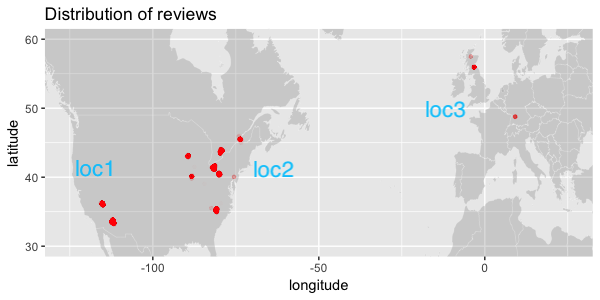
\includegraphics[scale=0.4]{../image/worldmap.png}
\end{frame}


\begin{frame}{2.2 Additional Variable}

\begin{itemize}
\item[-] \textbf{S1 $\sim$ S5}: S1[word] = $\frac{\text{P(this word is included in reviews with 1 star)}}{\text{P(this word is included in reviews with other stars)}}$
\end{itemize}

\begin{table}[ht]

\centering % used for centering table
\begin{tabular}{l l r r r r r r} % centered columns (4 columns)
	\hline %inserts double horizontal lines
	Word   &Variable  & 1-star & 2-star & 3-star & 4-star & 5-star  \\ [0.5ex] % inserts table
	%heading
	\hline % inserts single horizontal line
	\textbf{refund}         & frequence   & 115    & 15     & 7      & 4      & 2      \\
	& probability & 0.011  & 0.002  & 0      & 0      & 0      \\
	& S1 $\sim$ S5     & 34.200 & 1.080  & 0.300  & 0.072  & 0.025  \\
	\hline
	\textbf{notdisappoints} & frequence   & 0      & 2      & 5      & 43     & 110   \\
	& probability & 0      & 0      & 0      & 0.002  & 0.003  \\
	& S1 $\sim$ S5     & 0      & 0.116  & 0.188  & 0.917  & 3.870  \\
	\hline
	\textbf{and}            & frequence   & 9196   & 8691   & 12851  & 25604  & 32071  \\
	& probability & 0.859  & 0.886  & 0.877  & 0.895  & 0.886  \\
	& S1 $\sim$ S5     & 0.968  & 1.000  & 0.991  & 1.020  & 1.000  \\
	
	\hline %inserts single line
\end{tabular}
\label{table:nonlin} % is used to refer this table in the text
\end{table}

\end{frame}

% 4-----------------------------------------------------------------------------------
\begin{frame}{4 Compare RMSE with other method}

\begin{table}[]
\centering
\caption*{\huge{RMSE}}

\begin{tabular}{lrrrrrr}
Feature$\backslash$ Model & GLM   & LM & SVM & NB & LSTM & NN \\
\hline
frequence     & 0.864 & 0  & 0   & 0  & 0    & 0  \\
tf-idf        & 0.836 & 0  & 0   & 0  & 0    & 0  \\
vector        & 0     & 0  & 0   & 0  & 0    & 0  \\
ad            & 0     & 0  & 0   & 0  & 0    & 0  \\
vector + ad   & 0     & 0  & 0   & 0  & 0    & 0 \\
\hline
\end{tabular}
\label{table:nonlin} 
\end{table}

\end{frame}


\begin{frame}
\Huge{\centerline{Thank You!}}
\end{frame}
\end{document}
